\documentclass[11pt,ngerman]{article}
\usepackage{geometry}
\usepackage[T1]{fontenc}
\usepackage[utf8]{inputenc}
\usepackage{babel}
\usepackage{hyperref}
\usepackage{lmodern}%get scalable font
\usepackage{titling}
\usepackage{relsize}
\usepackage{biblatex}
\usepackage{glossaries}
\usepackage{paralist}
\usepackage[table, dvipsnames]{xcolor}
\usepackage{booktabs}
\usepackage{tabularx}
\usepackage{float}
\restylefloat{table}
\usepackage{setspace}
\usepackage{multicol}
\usepackage{graphicx}
\usepackage[space]{grffile}
\usepackage[most]{tcolorbox}
\usepackage{enumitem}
\usepackage{textcomp}
\usepackage{listings}


% Link colors
\hypersetup{
    colorlinks,
    linkcolor={blue},
    citecolor={red},
    urlcolor={blue}
}

\geometry{a4paper, top=25mm, left=25mm, right=25mm, bottom=20mm,
    headsep=10mm, footskip=12mm}

% inline code macro
\definecolor{lightgray}{gray}{0.9}
\lstset{
    showstringspaces=false,
    basicstyle=\ttfamily,
    keywordstyle=\color{blue},
    commentstyle=\color[grey]{0.6},
    stringstyle=\color[RGB]{255,150,75}
}
\newcommand{\inlinecode}[2]{\colorbox{lightgray}{\lstinline[language=#1]$#2$}}

% Glossary
% Das Glossar definiert alle wichtigen Begriffe zur Sicherstellung einer einheitlichen Terminologie.
% Es sollen keine allgemeinen Begriffe erklärt werden, die den Adressaten bekannt sind (z. B. Java, CPU etc.).

\pretitle{\begin{center}\linespread{1.5}\huge}
    \posttitle{\par\end{center}\vspace{0.5em}}

% double quotes macro
% usage: \quotes{arg1}  => in text: "arg1"
\newcommand{\quotes}[1]{``#1''}

\begin{document}

    \title{Tron Licht-Motorräder Computerspiel\\
        \vspace{1cm}
        Bedienungsanleitung \\
        \vspace{0.5cm}
        \small{}ZHAW  School of Engineering
        \vspace{1.5cm}
    }
    \author{
        Akca, Deniz\\
        \small{akcaden1@students.zhaw.ch}
        \and
        Holenstein, Christian\\
        \small{holenchr@students.zhaw.ch}
        \and
        Huber, Patrick\\
        \small{huberpa4@students.zhaw.ch}
        \and
        Iten, Mike\\
        \small{itenmik1@students.zhaw.ch}
        \vspace{1.5cm}
    }
   \date{\today}

    \maketitle
    \newpage

    \tableofcontents
	\listoffigures
    \newpage
    
    \section{Beschreibung}
    
    Ein Spieler besitzt ein sogenanntes Licht-Motorrad. Dieses zieht während der Fahrt eine Linie nach sich, die bestehen bleibt. Fährt ein Spieler in eine dieser Linien, scheidet dieser aus. Gewinner ist, wer im Spiel bleibt, bis alle anderen Spieler ausgeschieden sind.
    
    \section{Anmeldung}
    
    Dem User stehen verschiedene Möglichkeiten zur Verfügung. Durch das erstmalige Betreten wird der User automatisch als Gast angemeldet --1-- und kann direkt einem Spiel beitreten oder ein Spiel erstellen. 
    Falls der User sich registrieren möchte um Punkte für die Statistik zu sammeln, so hat er hier die Möglichkeit dazu --2--. 
    
    \begin{figure}[H]
    	\centering
    	\makebox[\textwidth][c]{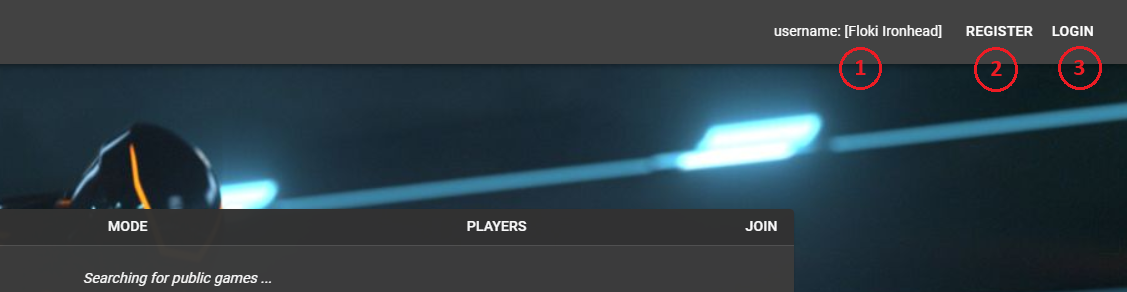
\includegraphics[width=0.95\textwidth]{figures/Anmeldung.png}}
    	\caption{Anmeldung}
    	\label{fig:Anmeldung}
    \end{figure}
    
    Sollte bereits ein Account vorhanden sein, dann ist der Login hier --3-- vorzufinden.
       
    \begin{figure}[H]
    	\centering
    	\makebox[\textwidth][c]{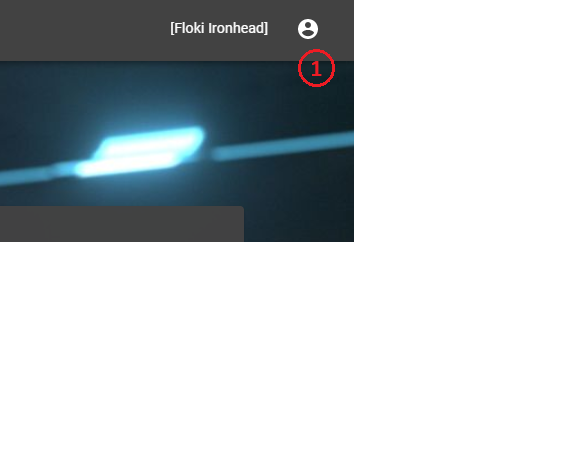
\includegraphics[width=0.95\textwidth]{figures/MyAccount.png}}
    	\caption{MyAccount}
    	\label{fig:MyAccount}
    \end{figure}

	Nach erfolgreicher Anmeldung kann der User bei MyAccount --1-- seine verschiedenen Daten einsehen oder ändern. 
    
    \section{Spielablauf}
    
    
    \subsection{Lobby beitreten}
    
    Der User kann über den Button 1 einer Lobby beitreten, dies ist nur für Lobbys möglich, welche mit der Eigenschaft Public erstellt wurden.
    
    \begin{figure}[H]
    	\centering
    	\makebox[\textwidth][c]{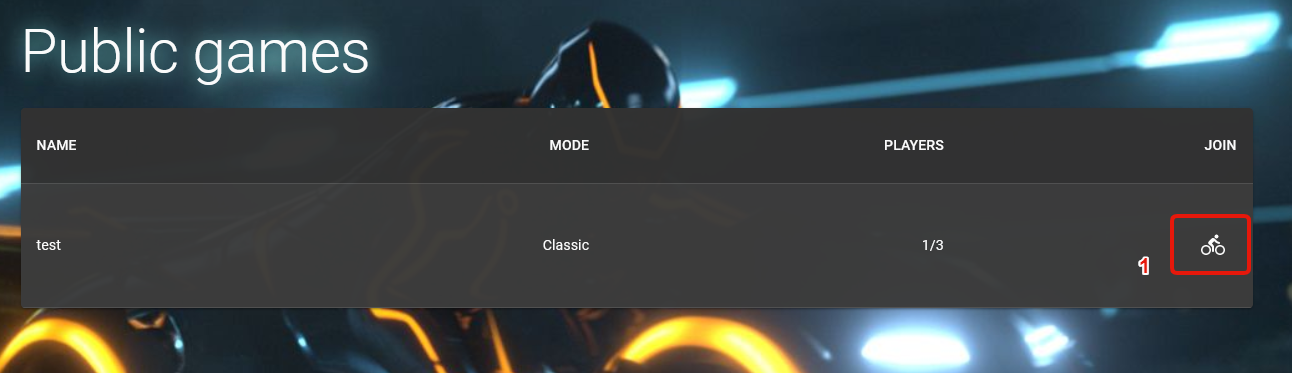
\includegraphics[width=0.95\textwidth]{figures/Spiel_beitreten.png}}
    	\caption{Spiel beitreten}
    	\label{fig:Spiel_Beitreten}
    \end{figure}
    
    \subsection{Lobby erstellen}
    
    Wenn der User eine eigene Lobby erstellen möchte, dann hat er in dem folgenden Bild die Möglichkeit dazu.
    
	\begin{figure}[H]
		\centering
		\makebox[\textwidth][c]{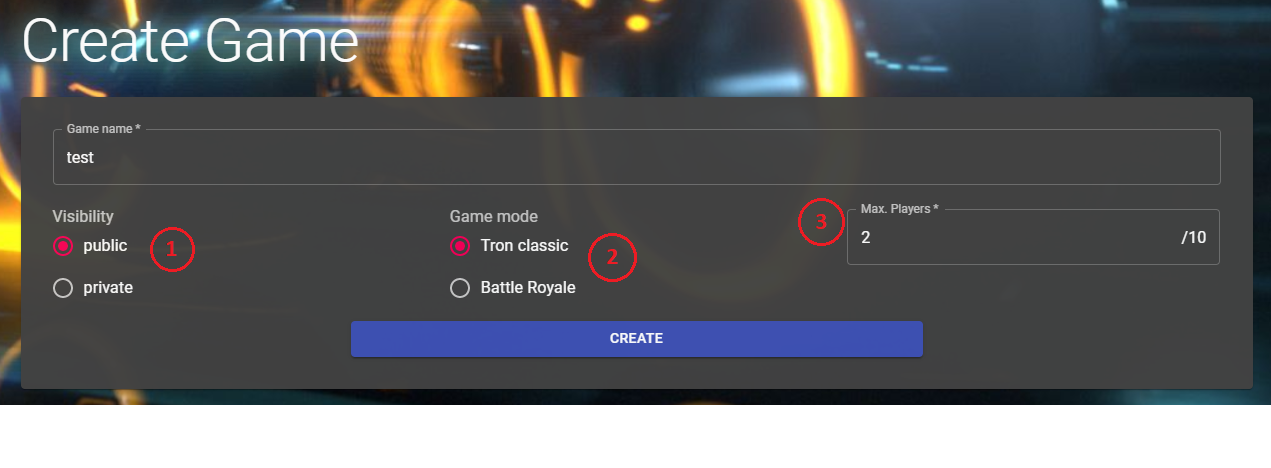
\includegraphics[width=0.95\textwidth]{figures/Spiel_erstellen.png}}
		\caption{Spiel erstellen}
		\label{fig:Spiel_Erstellen}
	\end{figure}
    
    --1-- Wird die public Eigenschaft ausgewählt, dann wird die Lobby unter Public Games aufgeführt. 
    
    --2-- Tron classic ist der Standardmodus, welcher ein klassisches Spiel darstellt. Dies beinhaltet ein Maximum von bis zu 10 Spielern. Battle Royale erstellt ein Spiel, welches 100 Spieler beinhalten muss.
    
    --3-- Dies indiziert wie viele Spieler der Lobby beitreten dürfen. Sobald das Limit erreicht ist, können keine weiteren Spieler beitreten.
    
	\subsection{Lobby}
	
	Sobald eine Lobby erstellt oder einer beigetreten wurde, sollte der folgende Ausschnitt ersichtlich sein.
    \begin{figure}[H]
    	\centering
    	\makebox[\textwidth][c]{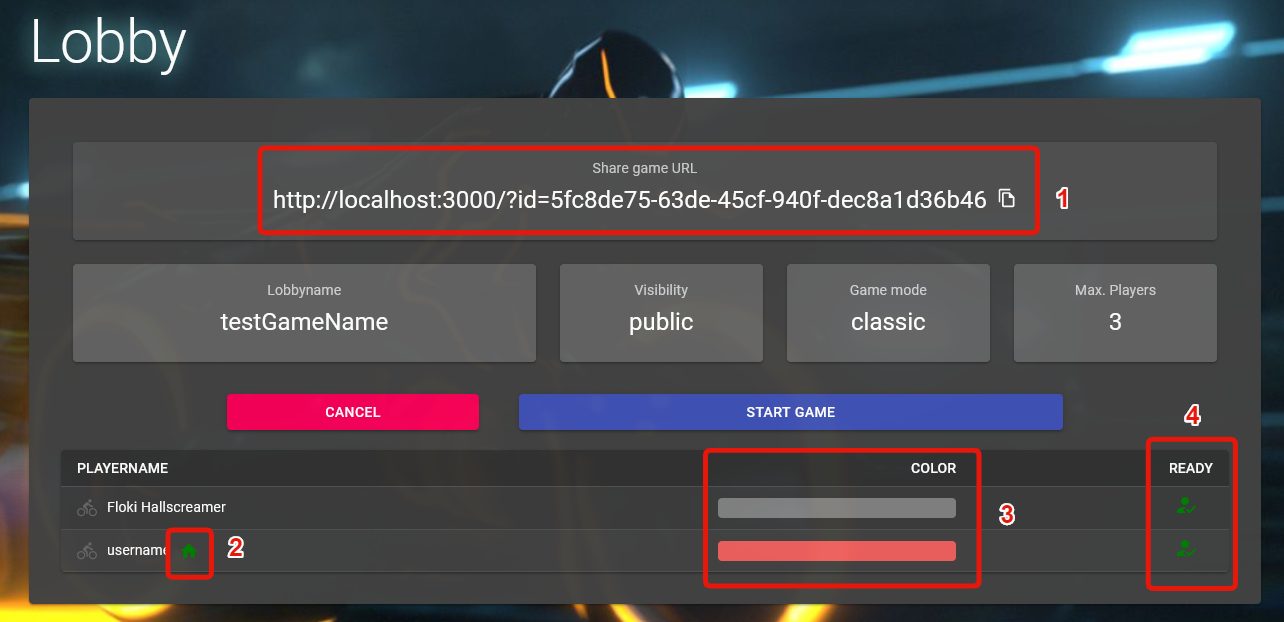
\includegraphics[width=0.95\textwidth]{figures/Lobby.png}}
    	\caption{Lobby}
    	\label{fig:Lobby}
    \end{figure}
  
    
    --1-- Dieser URL kann kopiert werden und an einen Freund gesendet werden. Dieser kann den URL in den Browser kopieren und tritt somit nach Bestätigung eines Fensters der Lobby bei.
    
    --2-- Das grüne Haus signalisiert, welcher Spieler der Ersteller der Lobby ist und somit das Spiel starten kann.
    
    --3-- Die Farbe wurde von der Registrierung übernommen und kann im Profil geändert werden.
    
    --4-- Sobald alle Spieler ein grünes Symbol haben, bedeutet das, dass der Ersteller der Lobby das Spiel starten kann
    
    \subsection{Spielen}
    
    Nachdem der Lobbyersteller auf Start Game geklickt hat, erscheint ein Spielfeld und ein Countdown zählt runter.
    
    \begin{figure}[H]
    	\centering
    	\makebox[\textwidth][c]{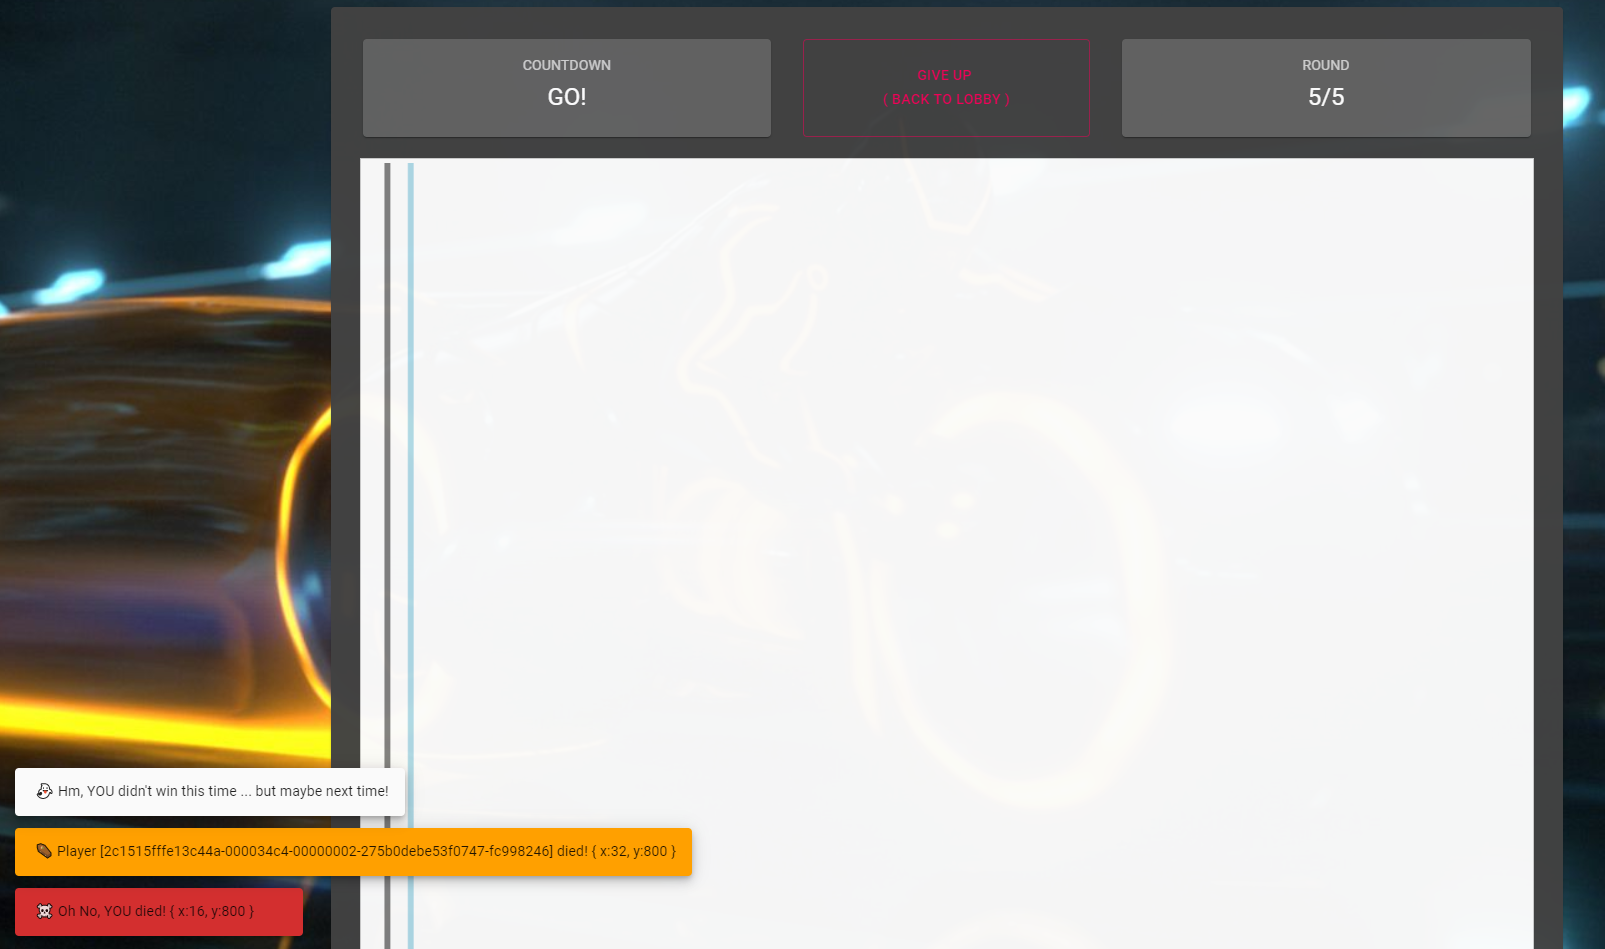
\includegraphics[width=0.95\textwidth]{figures/Spielfeld.png}}
    	\caption{Spielfeld}
    	\label{fig:Spielfeld}
    \end{figure}
    
    Mit den Pfeiltasten kann das Motorrad in die jeweiligen Richtungen navigiert werden. 
    Hierbei ist zu beachten, dass die eigene Linie und die Linie anderer Spieler zu vermeiden ist. Desweiteren scheidet man aus, sobald das Motorrad aus dem Spielfeld fährt. 
    Schlussendlich ist das Ziel der letzte Spieler auf dem Feld zu sein. Nach 5 Runden ist ein Spiel vorbei. Nach jeder Runde erscheint eine Nachricht, ob man gewonnen oder verloren hat.
   
    
\end{document}